\documentclass{article}

\usepackage[most]{tcolorbox}
\usepackage{physics}
\usepackage{graphicx}
\usepackage{float}
\usepackage{amsmath}
\usepackage{amssymb}


\usepackage[utf8]{inputenc}
\usepackage[a4paper, margin=1in]{geometry} % Controla los márgenes
\usepackage{titling}

\title{Talle \#1 de metodos geometricos}
\author{Manuel Garcia, Carlos Andres Llanos}
\date{\today}

\renewcommand{\maketitlehooka}{%
  \centering
  \vspace*{0.05cm} % Espacio vertical antes del título
}

\renewcommand{\maketitlehookd}{%
  \vspace*{2cm} % Espacio vertical después de la fecha
}

\newcommand{\caja}[3]{%
  \begin{tcolorbox}[colback=#1!5!white,colframe=#1!25!black,title=#2]
    #3
  \end{tcolorbox}%
}

\begin{document}
\maketitle

\section{Ejercicio 1 de la seccion 1-3 del Do Carmo}
Mostrar que las lineas tangentes a la curva regular parametrizada $ \alpha(t) = (3t,3t ^2, 2t ^ {3 }) $ forman un angulo constante con $ y = 0  $ y $ z = x  $. 
\textbf{Sol.} Tenemos entonces que $ \alpha(t) = (3t,3t ^2, 2t ^ {3 }) $, $ \beta(t) = (t,0,t) $ y $ \phi(t) = (t,t,3t) $ asumiendo cada recta independiente calculando los vectores velocidad de cada curva tenemos: 
\begin{gather*}
  \alpha'(t) = (3, 6t, 6t ^2), \qquad \beta'(t) = (1,0,1), \phi(t) = (1,1,3) 
\end{gather*}
Donde sabemos que el ángulo entre dos curvas que se interceptan es: 
\begin{gather*}
  \cos{\theta} = \frac{\bra{\alpha' }\ket{\beta' } }{\sqrt{\bra{\alpha' }\ket{\alpha' } \bra{\beta' }\ket{\beta' } } }
\end{gather*}

entonces: 

\begin{gather*}
  \bra{\alpha'}\ket{\beta' } = 3 + 6t ^2, \qquad \bra{\beta' }\ket{\beta'} = 2, \qquad \bra{\alpha' }\ket{\alpha' } = 9 + 36t ^2 + 36t ^ {4 }\\
\cos{\theta} = \frac{3+ 6t ^2}{\sqrt{9 + 36t ^2 + 36 t ^ {4 }} }\frac{\sqrt{2 } }{2}\\
\text{Resolviendo la raiz del denominador: }\\
\sqrt{9 + 36 t ^2 + 36 t ^ {4 }}  = 3 \sqrt{1 + 4 t ^2 + 4 t ^ {4 }} \\
\text{Tomando }t ^2 = u \text{ y simplificando: }\\
1 + 4 u + 4 u ^2 = 2u (1 + 2u) + (1+ 2u ) = (2u + 1)(2u+ 1) = (2u + 1)^2\\
\text{Entonces tenemos que: }\\
\cos{\theta} = \frac{3 + 6 t ^2 }{3(2t ^2+ 1)}\frac{\sqrt{2 } }{2} = \frac{\sqrt{2 } }{2}
\end{gather*}

Entonces tenemos que $ \theta = \cos^ {-1 }{\frac{\sqrt{2 } }{2}} = \frac{\pi}{4}k  $ con $ k \in \mathbb{Z} $, el angulo $ \theta  $ es constante ya que $ \beta(t) $ es una funcion suave y $ \alpha(t)  $ con $ t>0  $ son suaves ya que $ \alpha'(t) \neq 0  $ y $ \left|\alpha'(t)\right|\neq 0 $

\section{Ejercicio 2 de la seccion 1-3 del Do Carmo }
Un disco circular de radio 1 en el plano $ xy  $ rueda sin deslizarce a lo largo del eje x. La figura descrita por un punto de la circunferencia del disco es llamada cicloide. 
\begin{figure}[H]
  \begin{center}
    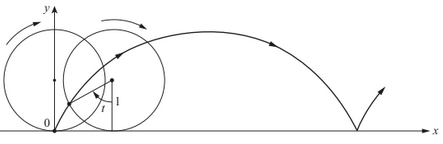
\includegraphics[width=0.6\textwidth]{figures/cicloide-do-carmo.png}
  \end{center}
  \caption{Cicloide}
  \label{fig:cicloide}
\end{figure}
Tenemos la parametrizacion: $ x ^ {1 } = L - \sin{\alpha}, \quad x ^ {2 } = 1- \cos{\alpha} $. Si usamos la ligadura de rodadura tenemos que $ L = r \alpha = \alpha $. Entonces: 
\begin{gather*}
  P = (\alpha - \sin{\alpha}, \quad 1 - \cos{\alpha}) = (t - \sin{t}, \quad 1 - \cos{t})
\end{gather*}

\textbf{a) }Los puntos singulares serán donde el determinante de $ a_j = \left. \left(\frac{\partial x'  }{\partial z ^ {j }}\right)\right|_{z' = z'_0}  $ sea distinto de 0. 

Derivando $ x = x(x ^ {1 }, x ^ {2 }), \quad z = z(r,\alpha), \quad r = 1  $. 
\begin{gather*}
  a_1 ^ {1 } = \frac{\partial \alpha-\sin{\alpha} }{\partial r} = 0 , \qquad \quad a _{2 } ^ {1 } = \frac{\partial \alpha- \sin{\alpha} }{\partial \alpha} = 1- \cos{\alpha}\\
  a _{1 } ^ {2 } = \frac{\partial r - \cos{\alpha} }{\partial r} = 1, \qquad \quad a _{2 } ^ {2 } = \frac{\partial 1- \cos{\alpha} }{\partial \alpha} = \sin{\alpha}\\
  \left|a _{j } ^ {i }\right| = \left|\begin{bmatrix}
      0 & 1-\cos{\alpha} \\
      1  & \sin{\alpha}
  \end{bmatrix}  \right|
\end{gather*}
Entonces para conocer qué puntos se anulan $ 1- \cos{\alpha} = 0 \rightarrow \alpha = \cos^ {-1}{1 } $

Tenemos que si $ \alpha = n \pi, \quad n\in \mathbb{Z}, \quad \left|a _{j } ^ {i }\right| = 0  $

\textbf{b) } Parametrizando con $ u = t  $ tenemos: 
\begin{gather*}
  P =  r(t - \sin{t }, \quad 1- \cos{t }); \qquad \vec v (t) = r (1 - \cos{t }, \quad \sin{t }) \\
  \bra{v(t)}\ket{v(t)} = r ^2 - 2 r \cos{t } + \cos ^2{t} + \sin ^2{t}\\
  = r ^2 - 2 r \cos{t } + 1, \quad \text{pero con }r = 1: \\
  = 2 - 2 \cos{t }\\
  S = \int_{0 }^{2 \pi}\sqrt{2 - 2 \cos{t }} dt = 8 
\end{gather*}

\section{Ejercicio 6 de la seccion 1-3 del Do Carmo }
Sea $ \alpha(t) = (a e ^ {bt }\cos{t }, a e ^ {b t } \sin{t }), \quad t \in \mathbb{R} $, $ a  $ y $ b  $ constantes, $ a > 0  $, $ b <0  $, una curva parametrizada
\textbf{a) } muestre que $ \alpha(t) = (a e ^ {b t } \cos{t }, a e ^ {bt } \sin{t }) $ es una espiral que cuando $ t \rightarrow + \infty $ se aproxima al origen 
\textbf{Sol. } 
\begin{gather*}
  r(t) = a e ^ {bt } 
\end{gather*}
donde r es el radio que depende de un angulo $ t  $. Como $ b<0  $ y $ a >0  $ podemos escribirlo como: 
\begin{gather*}
  r(t) = \left|a \right|e ^ {-\left|b \right|t }
\end{gather*}
entonces 
\begin{gather*}
  \underset{t \rightarrow \infty}{lim }\left|a \right|e ^ {- \left|b \right|t } = 0  
\end{gather*}
Por lo que se aproxima al origen.

\textbf{b) }
\begin{gather*}
  \underset{t \rightarrow \infty}{lim }\int_{t_0 }^{t } \left|\alpha'(t)\right|dt 
\end{gather*}
\begin{align*}
  \alpha(t) &= (a e ^ {bt }\cos{t }, a e ^ {bt }\sin{t })\\
  \alpha' (t) &= (a b e ^ {bt }\cos{t }- a e ^ {bt } \sin{t },\quad ab e ^ {bt } \sin{t }+ a e ^ {bt } \cos{t })\\
  \left|\alpha' (t) \right| &= \sqrt{(a b e ^ {bt }\cos{t }- a e ^ {bt } \sin{t }) ^2 + (ab e ^ {bt } \sin{t }+ a e ^ {bt } \cos{t })^2} \\
  &= \sqrt{a ^2 c ^2 e ^ {2bt } + a ^2 e ^ {2bt }} \\
  &= \sqrt{a ^2 e ^ {2bt }(1 + b ^2)} \\
  &= a e ^ {bt } \sqrt{1 + b ^2} 
\end{align*}

\begin{gather*}
  l(t) = \underset{t \rightarrow \infty}{lim }\int_{t_0 }^{t } a \sqrt{1 + b ^2} e ^ {bt } dt \\
  l = \underset{t \rightarrow \infty}{lim }\frac{a}{b} \sqrt{1 + b ^2}  e ^ {bt }\\
  l = - \frac{a}{b} \sqrt{b ^2 + 1 }  e ^ {bt_0}
\end{gather*}

\section{Ejercicio 1 de la parte 2 }
Calcule las componentes de la métrica en $ \mathbb{R}^ {3 } $ en coordenadas esféricas.

\textbf{Sol. } 
\begin{gather*}
  x = r \cos{\phi }\sin{\theta}\\
  y = r \sin{\phi }\sin{\theta}\\
  z = r \cos{\theta}\\
  g _{ij }  = \delta _{ij } \frac{\partial x ^ {k } }{\partial z ^ {i }} \frac{\partial x ^ {l } }{\partial z ^ {i }}\\
  \frac{\partial x ^ {k } }{\partial z ^ {i }} = \begin{bmatrix}
      \cos{\phi }\sin{\theta} & r \cos{\phi }\cos{\theta} & - r \sin{\phi }\sin{\theta} \\
      \sin{\phi }\sin{\theta} & r \sin{\phi }\cos{\theta} & r \cos{\phi }\sin{\theta} \\
      \cos{\theta} & -r \sin{\theta} & 0 
  \end{bmatrix} 
\end{gather*}

\begin{gather*}
  g _{11 }  = \delta _{11 } \frac{\partial x  }{\partial r }\frac{\partial x  }{\partial r } + \delta _{11 } \frac{\partial y  }{\partial r}\frac{\partial y  }{\partial r } + \delta _{11 }  \frac{\partial z  }{\partial r} \frac{\partial z  }{\partial r }\\
  = \sin ^ {2 }{\theta } + \cos ^2{\theta }\\
  = 1
\end{gather*}

\begin{gather*}
  g _{22 }  = \delta _{22 } \frac{\partial x  }{\partial \theta }\frac{\partial x  }{\partial \theta } + \delta _{22 } \frac{\partial y  }{\partial \theta}\frac{\partial y  }{\partial \theta } + \delta _{22 }  \frac{\partial z  }{\partial \theta} \frac{\partial z  }{\partial \theta }\\
  = r ^2(\sin ^ {2 }{\theta } + \cos ^2{\theta })\\
  = r ^2
\end{gather*}

\begin{gather*}
  g _{33 }  = \delta _{33 } \frac{\partial x  }{\partial \phi }\frac{\partial x  }{\partial \phi } + \delta _{33 } \frac{\partial y  }{\partial \phi}\frac{\partial y  }{\partial \phi } + \delta _{33 }  \frac{\partial z  }{\partial \phi} \frac{\partial z  }{\partial \phi }\\
  = r ^2 \sin ^2{\theta}
\end{gather*}

\begin{gather*}
  g _{ij }  = \begin{bmatrix}
      1 & 0 & 0 \\
      0 & r ^2 & 0 \\
      0 & 0 & r ^2 \sin ^2{\theta}
  \end{bmatrix}
\end{gather*}

\section{Ejercicio 2 de la parte 2 }
Calcule las componentes de la metrica en $ \mathbb{R}^ {3 }_{(1,2 )}  $ en coordenadas pseudo-esfericas $ (\rho, \chi,\phi) $
\begin{gather*}
  x ^ {0 } = \rho \cosh{\chi } \\
  x ^ {1 } = \rho \sinh{\chi }\cos{\phi} \\
  x ^ {2 } = \rho \sinh{\chi }\sin{\phi} 
\end{gather*}

\textbf{Sol. }

Para calcularlo usamos: 
\begin{gather*}
  g _{\mu \nu } = \frac{\partial x ^ {\alpha} }{\partial x ^ {\mu }}\frac{\partial x ^ {\beta} }{\partial x ^ {\nu}}\eta _{\alpha \beta}  
\end{gather*}
Donde $ \eta _{\alpha\beta} $ es la metrica de minkowski en el espacio $ \mathbb{R}^ {3 }_{(1,2)}  $
\begin{gather*}
  \eta _{\alpha\beta}  = \begin{bmatrix}
      1 & 0 & 0 \\
      0 & -1  & 0 \\
      0 & 0 & -1
  \end{bmatrix}  \\
  \begin{bmatrix}
      \cosh{\chi} & \rho \sinh{\chi } & 0  \\
      \sinh{\chi }\cos{\phi } & \rho \cosh{\chi }\cos{\phi } & \rho \sinh{\chi }\sin{\phi } \\
      \sinh{\chi }\sin{\phi } & \rho \cosh{\chi }\sin{\phi } & \rho \sinh{\chi }\cos{\phi}
  \end{bmatrix} 
\end{gather*}

\begin{align*}
  g _{11 }  &= \cosh ^ {2 }\chi - \sinh ^2 \chi \cos ^2{\phi} - \sinh{\chi }\sin{\phi }\\
  &= \cosh ^2 \chi - \sinh ^2 \chi \\
  &= 1
\end{align*}

\begin{align*}
  g _{22 }  &= \rho ^2\sinh ^ {2 }\chi - \rho ^2\cosh ^2 \chi \cos ^2{\phi} - \rho ^2\cosh ^2{\chi }\sin{\phi }\\
  &= \rho ^2(\sinh ^2 \chi-\cosh ^2 \chi) \\
  &= \rho ^2 
\end{align*}

\begin{align*}
  g _{33 }  &= \rho ^2\sinh ^ {2 }\chi\sin ^2 \phi  - \rho ^2\sinh ^2 \chi \cos ^2{\phi}\\
  &= - \rho ^2 \sinh ^2\chi
\end{align*}

\begin{gather*}
  g' _{ij }  = \begin{bmatrix}
      1 & 0 & 0 \\
      0 & -\rho ^2 & 0 \\
      0 & 0 & -\rho ^2 \sinh ^2\chi
  \end{bmatrix}
\end{gather*}

\end{document}
